%%% První kapitola

\chapter{Definice a vlastnosti Jonesova polynomu}
Cílem této kapitoly je definovat Jonesův polynom, dokázat jeho základní vlastnosti a popsat souvislost se závorkovým polynomem. Vycházíme z materiálů~\cite{cromwell2004knots, Adams2004, jones2005} a vypracování cvičení z těchto zdrojů.
\section{Základní pojmy}
Jonesův polynom je invariant nejen uzlů, ale také \emph{linků}, tedy více propletených uzlů. Pokud není řečeno jinak, pracujeme v textu s linky. \\
Při definování Jonesova polynomu je důležité rozlišovat mezi linkem a jeho \emph{diagramem}. Diagram je vhodné rovinné nakreslení určité linkové projekce, v němž je rozlišeno, jestli křížení vedou \emph{svrchu}, nebo \emph{zdola}. Každý link má nekonečně mnoho diagramů.
\\
V diagramu \emph{orientovaného} linku rozlišujeme křížení s \emph{kladnou} a se \emph{zápornou orientací}, viz obrázek~\ref{orientace}.

\begin{figure}[h]  

\centering 
\begin{subfigure}[t]{0.4\linewidth}\centering
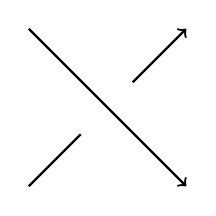
\begin{tikzpicture}[scale=2] 
\draw [thick] (0,0) -- (0.33,0.33);
\draw [thick,->] (0.66,0.66)-- (1,1);
\draw [thick,->] (0,1)  -- (1,0);
\end{tikzpicture} 
\caption{Kladná orientace.} 
\end{subfigure}
\begin{subfigure}[t]{0.4\linewidth}\centering
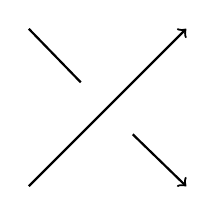
\begin{tikzpicture}[scale=2]
\draw [thick,->] (0,0) -- (1,1);
\draw [thick] (0,1) -- (0.33, 0.66);
\draw [thick,->] (0.66, 0.33) -- (1,0);
\end{tikzpicture}  
\caption{Záporná orientace.}
\end{subfigure}
\caption{Orientace křížení.} \label{orientace}
\end{figure}  


Pro popis polynomů na uzlech a lincích se často používají \emph{skein vztahy} \footnote{česky přadenové vztahy}.
Skein vztahy určují, jaká je spojitost mezi polynomy tří linků $L_+$, $ L_-$ a $L_0$, jejichž diagramy jsou identické až na oblast jednoho křížení. V linku $L_+$ má toto křížení kladnou orientaci, v $L_-$ zápornou a v $L_0$ je křížení rozpojené, viz obrázek~\ref{skein}.

\begin{figure}[h]  
\centering 
\begin{subfigure}[t]{0.4\linewidth}\centering
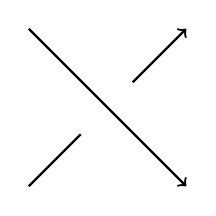
\begin{tikzpicture}[scale=2] 
\draw [thick] (0,0) -- (0.33,0.33);
\draw [thick,->] (0.66,0.66)-- (1,1);
\draw [thick,->] (0,1)  -- (1,0);
\end{tikzpicture} 
\caption{$L_+$} 
\end{subfigure}
\begin{subfigure}[t]{0.4\linewidth}\centering
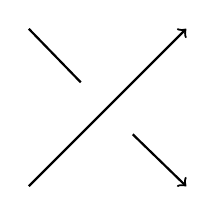
\begin{tikzpicture}[scale=2]
\draw [thick,->] (0,0) -- (1,1);
\draw [thick] (0,1) -- (0.33, 0.66);
\draw [thick,->] (0.66, 0.33) -- (1,0);
\end{tikzpicture}  
\caption{$L_-$}
\end{subfigure}
\begin{subfigure}[t]{0.4\linewidth}\centering
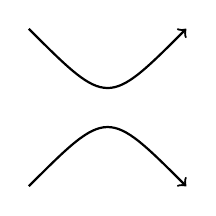
\begin{tikzpicture} [scale=2]
\draw  [thick,->](0,0) .. controls (1/2,1/2)  .. (1,0);
\draw  [thick,->](0,1) .. controls (1/2,1/2)  .. (1,1);
\end{tikzpicture}
\caption{$L_0$}
\end{subfigure}
\caption{Diagramy skein vztahu.} \label{skein}
\end{figure}

\section{Definice Jonesova polynomu}

\begin{definice}\label{def01:1}
\emph{Jonesův polynom} orientovaného linku $L$ je Laurentův polynom v~proměnné $\sqrt{t}$ (tj. polynom v $\Z[t^{1/2}, t^{-1/2}]$), značený $V_L(t)$ , který
\begin{enumerate}
\item
je linkový invariant,
\item 
  je normalizovaný, tedy polynom  $V_{\pmb{\circlearrowleft}}$ =1, kde ${\pmb{\circlearrowleft}}$ značí orientovaný triviální uzel,
\item  
splňuje skein vztah 
\begin{equation} \label{skein}
\frac{1}{t} V_{L_+} - t V_{L_-} = \left( \sqrt{t}  - \frac{1}{\sqrt{t}}\right) V_{L_0}.
\end{equation}
\end{enumerate}
\end{definice}

\begin{lemma}\label{l01:1}
Buď $L$ link, který se skládá z $k$ neprotínajících se orientovaných triviálních uzlů. Pak pro Jonesův polynom linku $L$ platí $$V_L(t) = \left(- \sqrt{t} -\frac{1}{\sqrt{t}}\right) ^{k-1}.$$
\end{lemma}
\begin{dukaz}
Libovolně orientované triviální uzly jsou navzájem ekvivalentní. Vzorec tedy stačí dokázat pro diagram skládající se z $k$ libovolně orientovaných disjunktních kružnic. Použijeme matematickou indukci.\\
Pro $ k=1$ vzorec platí podle druhé podmínky v definici ~\ref{def01:1}. \\
Předvedeme i případ, kdy $k = 2$. Pak $L_0 = $
\begin{tikzpicture}[line cap=round,line join=round,>=triangle 45,x=1cm,y=1cm, scale = 0.2]
\clip(-1.1,-1.1) rectangle (3.5,1.1);
\draw  (0,0) circle (1cm);
\draw  (2.38,0) circle (1cm);
\draw [line width=1/2pt] (0.6246950475544243,0.7808688094430303)-- (1,0.79);
\draw [line width=1/2pt] (0.6246950475544243,0.7808688094430303)-- (0.58,0.39);
\draw [line width=1/2pt] (1.7783415438306172,0.7987534676731457)-- (1.42,0.77);
\draw [line width=1/2pt] (1.7783415438306172,0.7987534676731457)-- (1.8,0.41);
\end{tikzpicture}, $L_- = $
\begin{tikzpicture}[line cap=round,line join=round,>=triangle 45,x=1cm,y=1cm, scale = 0.2]
\clip(-1.1,-1.1) rectangle (3.196466376386043,1.0990637767762312);
\draw [shift={(0,0)}]   plot[domain=0:5.105410206761974,variable=\t]({1*1*cos(\t r)+0*1*sin(\t r)},{0*1*cos(\t r)+1*1*sin(\t r)});
\draw [shift={(2,0)}]  plot[domain=-3.141592653589793:1.9340463984318206,variable=\t]({1*1*cos(\t r)+0*1*sin(\t r)},{0*1*cos(\t r)+1*1*sin(\t r)});
\draw [line width=0.5pt] (0.6222441255753678,0.7828232547561078)-- (1,0.78);
\draw [line width=0.5pt] (0.64,0.4)-- (0.6222441255753678,0.7828232547561078);
\end{tikzpicture}
 a $L_+ = $
\begin{tikzpicture}[line cap=round,line join=round,>=triangle 45,x=1cm,y=1cm, scale = 0.2]
\clip(-1.1403462213720332,-1.2) rectangle (3.0406984599653097,1.225538970539465);
\draw [shift={(0,0)}]  plot[domain=-5.158880748950075:0,variable=\t]({1*1.0280466904740395*cos(\t r)+0*1.0280466904740395*sin(\t r)},{0*1.0280466904740395*cos(\t r)+1*1.0280466904740395*sin(\t r)});
\draw [shift={(2,0)}]  plot[domain=-2.0668400051610742:3.141592653589793,variable=\t]({1*0.9664884893261791*cos(\t r)+0*0.9664884893261791*sin(\t r)},{0*0.9664884893261791*cos(\t r)+1*0.9664884893261791*sin(\t r)});
\draw [line width=0.5pt] (1.9692781611446357,0.6947891351587211)-- (1.977324654938205,0.966222453023282);
\draw [line width=0.5pt] (1.7119284298490884,1.200910273373297)-- (1.977324654938205,0.966222453023282);
\end{tikzpicture}. Diagramy $L_+$ a $L_-$ zobrazují triviální uzly, takže $V_{L_+} = V_{L_-} = 1$. Použitím skein vztahu získáme $$V_ L = V_{L_0} = - \sqrt{t} -\frac{1}{\sqrt{t}} .$$ \\
Pro $k > 2$ jsou $L_-$ a $L_+ $ diagramy linků s $k-1$ kružnicemi. Z indukčního předpokladu a ze skein vztahu získáme vzorec $$V_ L = V_{L_0} = \left(- \sqrt{t} -\frac{1}{\sqrt{t}}\right) ^{k-1}.$$
\end{dukaz}  

\begin{pozn}
Z každého uzlového diagramu lze změnou několika křížení vedených shora na křížení vedených zdola získat diagram triviálního uzlu. Z každého diagramu linku tedy můžeme změnou křížení získat diagram sjednocení triviálních uzlů, jejichž Jonesův polynom je podle předchozího lemmatu známý. Jonesův polynom každého linku lze tedy pomocí skein vztahu rekurzivně spočítat z jeho libovolného diagramu. Z toho plyno korektnost a jednoznačnost definice.
\end{pozn}


Definice Jonesova polynomu pomocí skein vztahů není vhodná pro algoritmický výpočet, neboť rozpoznat, jestli diagram odpovídá triviálnímu uzlu, je složitý problém. K výpočtu využijeme ekvivalentní definici založenou na použití \emph{závorkového polynomu}.

\section{Závorkový polynom}
Závorkový polynom \footnote{anglicky bracket polynomial nebo Kauffman bracket} je definován pouze pro diagramy neorientovaných linků, nikoli pro samotné linky.

\begin{definice}\label{def01:2}
\emph{Závorkový polynom} neorientovaného diagramu $D$, značený $\langle D \rangle$, je Laurentův polynom v proměnné $A$ definovaný třemi odvozovacími pravidly:
\begin{enumerate}
\item
$ \left\langle \pmb{\bigcirc} \right\rangle = 1$, kde $\pmb{\bigcirc}$ značí diagram s jednou komponentou bez křížení,
\item
$ \left\langle  \pluskriz
\right\rangle = A  \left\langle 
%vert
\vertkriz
 \right\rangle + A^{-1}  \left\langle
%hor 
\horkriz
\right\rangle $, kde~~\pluskriz~značí~~diagram obsahující toto křížení,~~\vertkriz~~je diagram, který je s ním shodný až na dané křížení, které je zde \emph{vertikální rozpojeno} a~~\horkriz~~je diagram, v němž je křížení \emph{rozpojeno horizontálně},
\item
$ \left\langle D \cup \pmb{\bigcirc} \right\rangle = (-A^2 - A^{-2}) \left\langle D \right\rangle$, kde $D \cup \pmb{\bigcirc} $ značí sjednocení diagramu $D$ a~diagramu s jednou komponentou bez křížení.
\end{enumerate}
\end{definice} 

\begin{pozn}
Pokud vztah v bodě \emph{2.} předchozí definice otočíme o 90°, získáme vztah
$ \left\langle
\minuskriz
\right\rangle = A  \left\langle
\horkriz
\right\rangle+ A^{-1} \left\langle
\vertkriz
\right\rangle $.
\end{pozn}

\begin{lemma}\label{l01:2}
Pro závorkové polynomy linků, jejichž diagramy obsahují smyčku, platí
\begin{enumerate}
\item
$ \left\langle 
%smycka 
\plussmycka
\right\rangle = -A^{-3} \left\langle 
\odsmycka
  \right\rangle$ 
\item
$ \left\langle 
\minussmycka
  \right\rangle = -A^{3} \left\langle 
\odsmycka
 \right\rangle$
\end{enumerate}
\end{lemma}

\begin{dukaz}
Použitím odvozovacích pravidel dokážeme první bod. 
\begin{equation*}
\left\langle
\plussmycka
 \right\rangle =  A \left\langle 
\odsmycka
\cup  \pmb{\bigcirc}   \right\rangle + A^{-1} \left\langle 
\odsmycka
 \right\rangle  = A (-A^2 - A^{-2}) \left\langle
\odsmycka
 \right\rangle + A^{-1}  \left\langle
\odsmycka
 \right\rangle  = -A^{-3} \left\langle
\odsmycka
 \right\rangle
\end{equation*}
Druhý bod se dokáže analogicky.
\end{dukaz}

Dva diagramy znázorňují stejný link (jsou ekvivalentní), pokud mezi nimi existuje série Reidemeisterových pohybů, viz obrázek~\ref{reid}. Z lemmatu ~\ref{l01:2} plyne, že závorkový polynom není invariantní vůči Reidemeisterovu pohybu typu I. Ukážeme, že je invariantní Reidemeisterovým pohybům typu~II a typu~III.

\begin{figure}[h]
\centering 
\begin{subfigure}{1\linewidth}\centering
\begin{tikzpicture}[scale = 0.70]
\clip(-2,-2) rectangle (7,1.3);
\draw (-1,1) .. controls (-2,2) and (-2,-2) .. (-1, -1);
\draw (-1,1) -- (1, -1);
\draw (-1,-1) -- (-0.25, -0.25);
\draw (0.25,0.25) -- (1,1);

\draw [thick, <->] (2,0) -- (3,0);

\draw (5,-1) arc (270:90:1);
\draw (5,-1) -- (7,-1);
\draw (5,1) -- (7,1);

\end{tikzpicture}
\caption{Typ I} 
\end{subfigure}
\begin{subfigure}{1\linewidth}\centering
\begin{tikzpicture}[scale = 0.70]
\clip(-2,-2) rectangle (7,1.3);

\draw (-1,-1) arc (270:90:1);
%\draw (-1, -1) -- (1, -1);
\draw (-1, -1) -- (-0.25, -1);
\draw (0.25, -1) -- (1, -1);
%\draw (-1, 1) -- (1, 1);
\draw (0, -1.3) -- (0, 1.3);
\draw (4, -1.3) -- (4, 1.3);

\draw (-1, 1) -- (-0.25, 1);
\draw (0.25, 1) -- (1, 1);

\draw [thick, <->] (2,0) -- (3,0);
\draw (5.5,-1) arc (270:90:1);
\draw (5.5,-1) -- (7,-1);
\draw (5.5,1) -- (7,1);

\end{tikzpicture} 
\caption{Typ II}
\end{subfigure}
\begin{subfigure}{1\linewidth}\centering
\begin{tikzpicture}[scale = 0.70]
\clip(-4.5,-1.65) rectangle (4.5, 1.65);

\draw [thick, <->] (-1/2,0) -- (1/2,0);

\draw (-4,1) -- (-3.58, 0.72);
\draw (-3.4, 0.6) -- (-1,-1);
\draw (-4, -1) -- (-3.58, -0.72);
\draw (-3.4, -0.6) -- (-2.8, -0.2);
\draw (-2.2, 0.2) -- (-1, 1);

\draw (1,-1) -- (2.2, -0.2);
\draw (2.8, 0.2) -- (3.4, 0.6);
\draw (3.58, 0.72) -- (4, 1); 
\draw (1,1) --  (3.4, -0.6) ;
\draw (3.58, -0.72) -- (4, -1);

\draw (-3.5, -1) -- (-3.5, 1);
\draw (3.5,-1) -- (3.5, 1);

\end{tikzpicture}
\caption{Typ III}
\end{subfigure}
\caption{Reidemeisterovy pohyby} \label{reid}
\end{figure}

\begin{tvrz}\label{t01:3}
Závorkový polynom je invariantní vůči Reidemeisterovým pohybům typu II a III.
\end{tvrz}
\begin{dukaz}
Použitím odvozovacích pravidel dokážeme invarianci vůči pohybu typu~II.
\begin{equation*}
\begin{split}
\left< \reiddva \right> & = A \left< \FO \right> - A^{-1} \left< \BO \right> \\ & = A \left( A \left< \DO \right> - A^{-1} \left< \EO \right> \right) \\ & - A^{-1} \left( A \left< \CO \right> - A^{-1} \left< \DO \right> \right) \\ & = \left< \CO \right> + \left( A^2 + A^{-2} \right) \left< \DO \right> + \left( -A^2 + -A^{-2} \right) \left< \DO \right>  \\ & = \left< \CO \right>
\end{split}
\end{equation*}
Invariance vůči pohybu typu III plyne z invariance vůči pohybu typu~II.
\begin{equation*}
\begin{split}
\left< \GO \right> & = A \left< \JO \right> - A^{-1} \left< \IO \right> \\ & = A \left< \JO \right> - A^{-1} \left< \KO \right>  \\ & = A \left< \JO \right> - A^{-1} \left< \LO \right> = \left< \HO \right>
\end{split}
\end{equation*}
\end{dukaz}

Aby byl závorkový polynom invariantní i vůči Reidemeisterovu pohybu typu~I, je nutné vynásobit jej výrazem, který vyjadřuje míru zakroucení.

\begin{definice}\label{def01:3}
\emph{Zakroucení} (writhe) orientovaného diagramu $D$ je součet znamení všech křížení v $D$. Zakroucení značíme $w(D)$.
\end{definice}

\begin{lemma}\label{l01:4}
Zakroucení je invariantní vůči Reidemeisterovým pohybům typu~II a~typu~III.
\end{lemma}
\begin{dukaz}
Důkaz se provede rozborem případů možných orientací křížení, která byla změněna daným Reidemeisterovým pohybem.
\end{dukaz}

\begin{definice}\label{def01:4}
\emph{Normalizovaný závorkový polynom} $X_L(A)$ orientovaného linku $L$ definijeme $$X_L(A) = (-A^3)^{-w(D)}\langle D \rangle,$$ kde $D$ značí libovolný diagram linku $L$.
\end{definice}

\begin{pozn}
Definice je korektní, neboť následující tvrzení ukazuje, že nezáleží na volbě diagramu.
\end{pozn}

\begin{tvrz}\label{t01:5}
Normalizovaný závorkový polynom je linkový invariant.
\end{tvrz}
\begin{dukaz}
Závorkový polynom i zakroucení jsou podle tvrzení~\ref{t01:3} a~lemmatu~\ref{l01:4} invariantní vůči Reidemeisterovým pohybům typu II a III, invariantní je tedy i jejich součin.

Invariance vůči typu I plyne z lemmatu~\ref{l01:2} a faktu, že křížení~\plussmycka~je vždy kladné a křížení~\minussmycka~vždy záporné.
\end{dukaz}

\begin{tvrz}\label{t01:6}
Při substituci proměnné $A = t^{-1/4}$ je normalizovaný závorkový polynom $X_L(A)$  roven Jonesovu polynomu $V_L(t)$.
\end{tvrz}
\begin{dukaz}
Ověříme, že $X_L(t^{-1/4})$ splňuje podmínky v definici~\ref{def01:1}:

\begin{enumerate}
\item
Normalizovaný závorkový polynom je podle předchozího tvrzení linkový invariant.
\item
Pro zamotání triviálního uzlu platí $w( \pmb{\bigcirc}) = 0$, tedy $$X_{\pmb{\circlearrowleft}} = (-A^3)^{w( \pmb{\bigcirc})} \langle \pmb{\bigcirc} \rangle = 1.$$ 
\item
Dokážeme ekvivalentní tvrzení, že $X_L(A)$ splňuje skein vztah~\ref{skein} při substituci $t=A^{-4}$. \\ Buď $L_+$, $ L_-$ a $L_0$ diagramy, pak platí
\begin{equation*}
\begin{split}
X_{L_+}(A) & = (-A^{-3})^{-w(L_+)} \langle L_+ \rangle = -A^{-3} (-A^3)^{-w(L_0)}  \langle \minuskriz  \rangle \\ & = -A^{-3} (-A^3)^{-w(L_0)} (A \langle \horkriz \rangle + A^{-1}  \langle \vertkriz \rangle)
\end{split}
\end{equation*}
\begin{equation*}
\begin{split}
X_{L_-}(A) & = (-A^{3})^{-w(L_-)} \langle L_- \rangle = -A^{3} (-A^3)^{-w(L_0)}  \langle \pluskriz  \rangle \\ & = -A^{3} (-A^3)^{-w(L_0)} (A \langle \vertkriz \rangle + A^{-1}  \langle \horkriz \rangle) .
\end{split}
\end{equation*}
Levá strana vztahu~\ref{skein} se tedy při substituci $t=A^{-4}$ rovná
\begin{equation*}
\begin{split}
A^4 X_{L_+}(t^{1/4})  - A^{-4} X_{L_-} (t^{1/4}) &  =  (-A^3)^{-w(L_0)} \left[ -A  (A \langle \horkriz \rangle + A^{-1}  \langle \vertkriz \rangle ) \right. \\ & \left. + A^{-1} (A \langle \vertkriz \rangle + A^{-1}  \langle \horkriz \rangle) \right] \\ & = (-A^3)^{-w(L_0)} (A^{-2} -A^2) \langle \horkriz \rangle \\ & =  (A^{-2} -A^2) X_{L_0},
\end{split}
\end{equation*}
což jsme měli dokázat.
\end{enumerate}
$ $
\end{dukaz}
